\begin{figure}[!t]
\centering
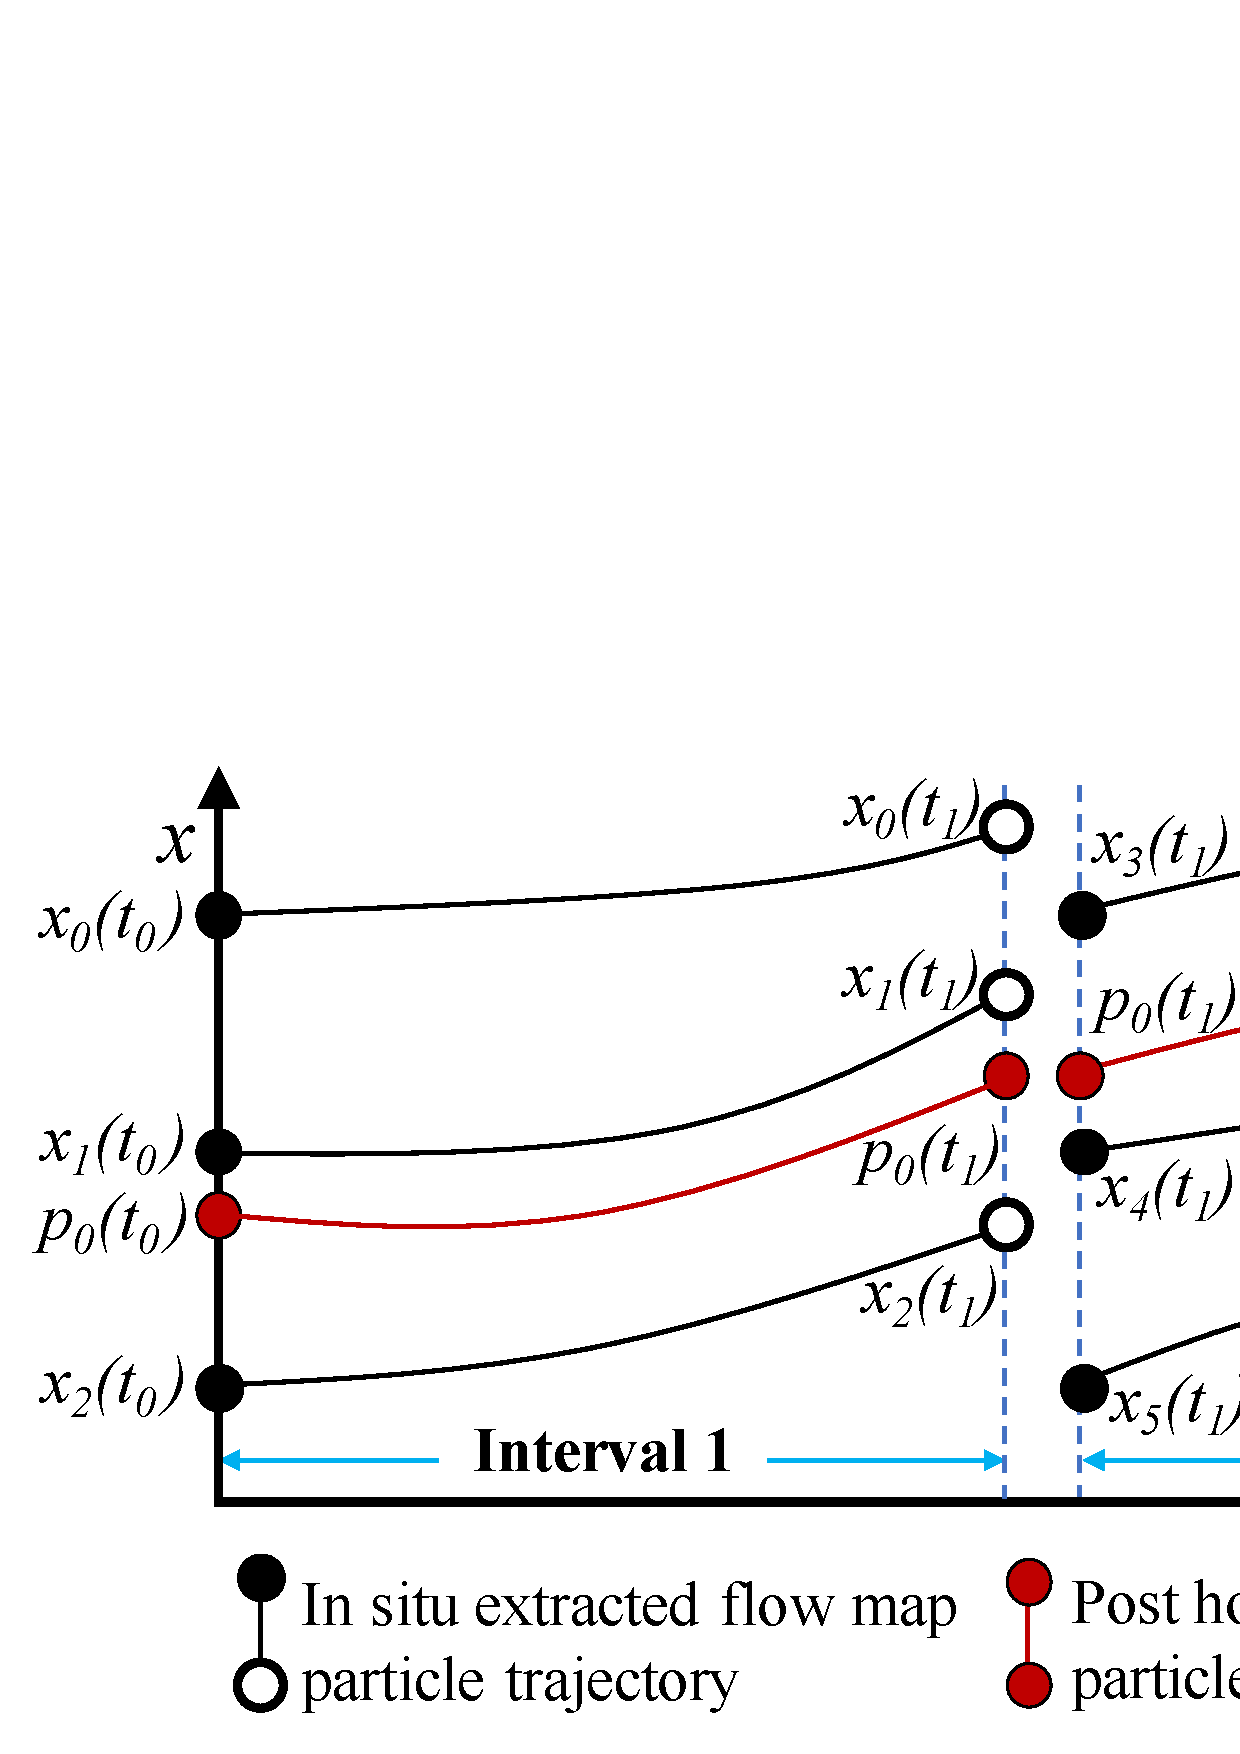
\includegraphics[width=\linewidth]{Images/phases_new_tall.pdf}
%\caption{\fix{The phases of Lagrangian analysis. The in situ phase uses uniform seed placement and extracts flow maps over temporally nonoverlapping intervals. In this example, the flow maps consist of particles \{$x_0$, $x_1$, $x_2$\} and \{$x_3$, $x_4$, $x_5$\} for the intervals [$t_0$, $t_1$] and [$t_1$,$t_2$], respectively. The flow maps are used as input during the post hoc phase. Here, the trajectory of particle $p_0$ is calculated by interpolating the flow maps over two intervals of time.}}
\caption{\fix{The phases of Lagrangian analysis. The in situ phase uses uniform seed placement and extracts flow maps over temporally nonoverlapping intervals. In this example, the flow map for the interval [$t_0$, $t_1$] consists of particles \{$x_0$, $x_1$, $x_2$\} and the flow map for the interval [$t_1$, $t_2$] consists of particles \{$x_3$, $x_4$, $x_5$\}. The extracted flow maps are used as input during the post hoc phase. Here, the trajectory of particle $p_0$ is calculated by interpolating the flow maps extracted over two intervals of time.}}
%\caption{\fix{The phases of Lagrangian analysis. The in situ phase uses uniform seed placement and extracts flow maps over temporally nonoverlapping intervals. In this example, the flow maps for [$t_0$, $t_1$] consist of \{$x_0$, $x_1$, $x_2$\} and for [$t_1$, $t_2$] consist of \{$x_3$, $x_4$, $x_5$\}. The extracted flow maps are used as input during the post hoc phase. In this example, the trajectory of particle $p_0$ is calculated by interpolating the flow maps extracted over two intervals of time.}}
\vspace{-6mm}
\label{fig:phases}
\end{figure}
